\documentclass[american,titlepage,oneside]{ntnuthesis}

\title{A modeling environment in the cloud for
education}
\shorttitle{Cloud modeling environment}
\author{Kristian Rekstad}
\shortauthor{K. Rekstad}
\date{\ntnuthesisdate}

\addbibresource{thesis.bib}


% From https://www.overleaf.com/learn/latex/Glossaries

\makeglossaries % Prepare for adding glossary entries


%\newglossaryentry{latex}
%{
%        name=latex,
%        description={Is a mark up language specially suited for
%scientific documents}
%}

%\newglossaryentry{bibliography}
%{
%        name=bibliography,
%        plural=bibliographies,
%        description={A list of the books referred to in a scholarly work,
%typically printed as an appendix}
%}

\newglossaryentry{Theia}
{
  name=Theia,
  description={An \acrshort{IDE} for software development. Theia is accessible in a web browser and as a desktop application. The implementation reuses much of \gls{VSCode}'s internals. Managed by the Eclipse Foundation.}
}

\newglossaryentry{VSCode}{
  name=VSCode,
  description={An \acrshort{IDE} for software development. The full name is Visual Studio Code. Managed by Microsoft.}
}

\newglossaryentry{metamodel}{
  name=metamodel,
  description={In conceptual modeling, the model itself can be modeled. This model of the model is called a meta-model. \Gls{Ecore} is one example of a metamodel.}
}

\newglossaryentry{Ecore}{
  name=Ecore,
  description={The \acrshort{emf} core model. A \gls{metamodel} similar to UML Class Diagrams.}
}

\newglossaryentry{Eclipse}{
  name={Eclipse IDE},
  description={An \acrshort{IDE} by the Eclipse Foundation. Originally created by IBM. It is based on a plugin architecture using OSGi, and is written in Java.}
}

% --------------------
% ----- Acronyms -----
% --------------------

%\newacronym{phd}{PhD}{philosophiae doctor}
%\newacronym{CoPCSE}{CoPCSE@NTNU}{Community of Practice in Computer ScienceEducation at NTNU}
%\newacronym{gcd}{GCD}{Greatest Common Divisor}

\newacronym{mdd}{MDD}{Model-Driven Development}
\newacronym{IDE}{IDE}{Integrated Development Environment}
\newacronym{emf}{EMF}{Eclipse Modeling Framework}
 % add glossary and acronym lists before document

\begin{document}

\chapter*{Abstract}

\Acrlong{mdd} is a an approach to software engineering.
A common framework for \gls{mdd} is the \acrlong{emf}.
However, students resist learning it because of its use of unpopular technologies.
This thesis comes before a master's thesis, and looks at how modeling can be moved to cloud based editors in order to renew the technology stack.
At the same time, opportunities for saving effort are found, by reusing existing implementations, architectures and protocols from other tools.
This thesis ends by finding the need for a tree based editor, and testing the feasibility of it.
Finally, some requirements and an architecture for such an editor are found.
These can be further studied and implemented in a master's thesis.
\chapter*{Sammendrag}


% TODO: write nor abstract


\tableofcontents
\listoffigures
\listoftables
\lstlistoflistings{}

\printglossary[type=\acronymtype] % Print acronyms
\printglossary{}                    % Print glossary


\chapter*{Acknowledgments}

\paragraph*{Hallvard Trætteberg} for being a very helpful supervisor
and for interesting discussions.

\paragraph*{Norwegian University of Science and Technology (NTNU)} for providing access to research papers, and for my education. 

\paragraph*{Jonas Helming} for providing answers about my research, and the initial title for the thesis.

% Melanie Bats
% Philip Langer

% Ingrid?
 
\chapter{Introduction}

\section{Context}

%Software engineering + modeling
\paragraph*{Software Engineering and Modeling}
Software engineering is a broad field. It has multiple approaches to methodology, programming languages, practices and paradigms.
One approach to developing software systems is to model a domain.
The domain is usually a phenomena in the real world which a business is interested in. And the conceptual model is an abstraction of this domain, where essential actors, entities, properties and relationships are formalized.

% MDSE, MDD, MBD
\paragraph*{Model usage}
This conceptual model can be utilized by the engineers to various degrees.
It could simply document the domain in order to help understanding and communication among those working with the domain. Or the model could be the basis of a software system. The software could be generated automatically based on the model, or an interpreting system could execute the model itself.

% MDD
\paragraph*{Model-Driven Development}
When the model itself is the source of truth for software, the model is \textit{driving} the development. This is called \acrfull{mdd}. Changes to the domain result in changes to the model, before changing the system's code. And the code itself is \textit{derived from the model}, often using model-to-text transformations. Oftentimes a \textit{complete} system can not be generated, and a programmer is required to manually code some details or rules of the domain into the generated code.

% Education of MDD
\paragraph*{Education and MDD}
The concepts and tools used in \acrshort{mdd} are being taught to software engineering students.
Not all curriculums include \acrshort{mdd}, as it is mostly relevant for specializations in Software Development. %Skip sentence?
Development using models is very reliant on tools. One of the tools that students learn is the \acrfull{emf} and its \gls{metamodel} called \gls{Ecore}.

% EMF details
\paragraph*{EMF in detail}
The \acrlong{emf} allows a modeller to create a representation of their domain, and generate java code. The java code has classes for all the modeled entities.
It can also generate an \textit{editor}, which is a user facing application.
This editor lets a user enter objects from their domain. For example, if the domain was a book store, the model would be \textit{books} with \textit{names} and \textit{authors}. And an object could be \textit{``Harry Potter''} by \textit{``J. K. Rowling''}. The generated editor uses \gls{Eclipse} as its platform, extending it with an \textit{Eclipse plugin}.

% Issues with EMF
\paragraph*{Issues with EMF}
Despite \acrshort{emf} being a great framework, its tight integration with \gls{Eclipse} harms the adoption. Some students have a negative attitude against \gls{Eclipse}, and learning about its architecture feels like wasted time.
\textcite{kuzniarzTeachingModelDrivenSoftware2016} found that students resist when the technology and skills are not used in other courses.
A general problem for \acrshort{mdd} adoption identified by \textcite{jonwhittleTaxonomyToolrelatedIssues2015} was a low impact on personal career needs. 
The students look to the industry, and mostly find mentions of ``IntelliJ, React, Typescript, Scrum, AI'', never Eclipse. They forget that much of the popular technologies are hype driven, and not the only tools used.
\textcite[p.~21--23]{brambillaModelDrivenSoftwareEngineering2017} claims that model-driven software engineering has passed the peak of the hype curve, and is now in the ``slope of enlightenment''. This means \acrshort{mdd} is not dead, but rather that we are only now seeing how it is best used.\footnote{Compare this to how the hyped Blockchain was supposed to fix every problem, but now we see it doesn't solve much at all.} One author of \cite{brambillaModelDrivenSoftwareEngineering2017} tried teaching students in 2015, and collected their feedback. Much of the complaints were about installation issues and problems with the tools. \cite{jordicabotFailedConvinceMy2015}


% My proposal


%TODO

% Related works and their shortcomings



\section{Stakeholders}

\paragraph*{Eclipse Foundation} They own and maintain the \acrlong{emf}, as well as \gls{Theia} and \gls{Eclipse}.

\paragraph*{Norwegian University of Science and Technology} They educate students in \acrlong{mdd}, and currently use \acrshort{emf}. Their lectures could use a cloud based modeling editor instead of \gls{Eclipse}.

% TypeFox
% EclipseSource
% RedHat
% Gitpods

\section{Research Questions}


\section{Scope}

% How the preproject is limited
This thesis is limited in scope, because it is part of a specialization project.
The main purpose of the thesis is to research and explore the background material. The research questions in \cref{chap:research-questions} will be refined from this exploration.
Some software development will be done, but the goal will be determining feasibility and discovering potential problems for a final solution.
The development will mainly be exploratory prototyping.

% How the preproject is comes before a master, and will aim to solve just a part of the problems.
%TODO: write

\section{Overview}

% Broad overview of the ecosystem,
% before diving into detail

An overview of the background material is shown in \cref{fig:background-overview}, before diving into it.
The figure is not optimal with respect to readability, but it illustrates that many of the items are related.
Not all relations are shown either, to maintain \emph{some level} of readbility.

\begin{figure}[htbp]  % order of priority: h here, t top, b bottom, p page
  \centering
  \hspace*{-2cm}%
  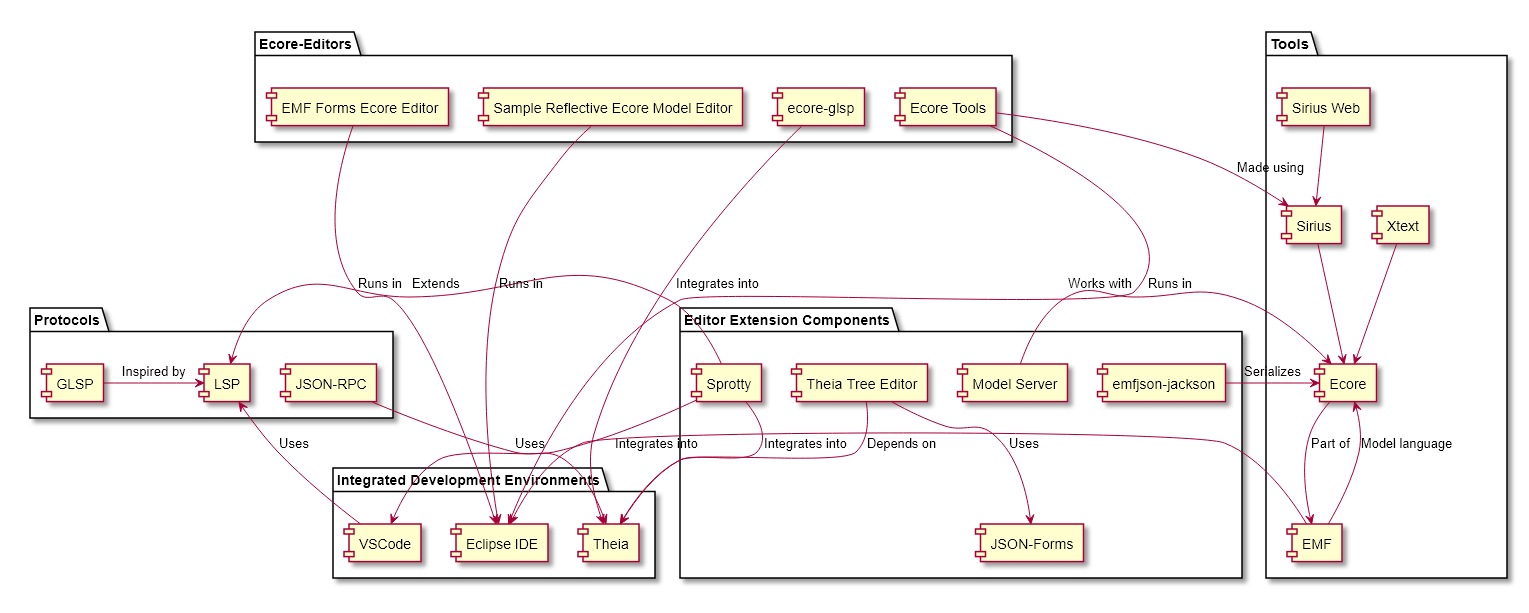
\includegraphics[width=1.4\textwidth]{figures/background-overview}
  \caption[Background Overview]{An overview of how the background is related.}\label{fig:background-overview}
\end{figure}

\chapter{Background}\label{chap:background}

\section{The Open Source Ecosystem}

Most of the work related to \acrlong{emf} is done as \gls{open source}.

\subsection{Co-opetition}

% core emf platform but competing tools

% Obeo+SiriusWeb+ObeoDesigner competes with EclipseSource+EMF.Cloud+GLSP
% Theia competes with VSCode
% Che competes with Gitpod

\subsection{Actors}

This section will present some of the main actors in the \acrlong{emf} ecosystem.
Most of the technologies discussed in \cref{sec:technologies} are developed by these actors.

% TODO: fill in actor descriptions

\paragraph*{Obeo} % Sirius, Eclipse Ecore Tools

\paragraph*{EclipseSource} % EMF Forms, JSON Forms, EMF Json? GLSP, Sprotty, Theia

\paragraph*{Eclipse Foundation} % EMF, Theia

\paragraph*{TypeFox} % Theia, Gitpod, Sprotty

\paragraph*{RedHat} % Che, Theia

\paragraph*{Microsoft} Not a part of \acrshort{emf}, but develops \gls{VSCode}. They decide which \acrshortpl{API} to support (which \gls{Theia} may have to implement).
Microsoft do not consider the \acrshort{emf} or \gls{Theia} developers when  making choices. % VSCode


\section{Technologies}\label{sec:technologies}

\subsection{Tools for Model-Driven Development}

This section will describe the most relevant tools when doing \acrfull{mdd} in the \acrlong{emf} ecosystem.

\subsubsection{Eclipse Modeling Framework and Ecore}

% What is Ecore
\paragraph*{What it is}
The \acrfull{emf} project provides tools for modeling and code generation.
\Acrshort{emf} consists of three main parts: an \emph{EMF core}, \emph{EMF.edit} and \emph{EMF.codegen}.
The core has a \gls{metamodel}, \emph{Ecore}, and a java runtime with support for change notifications, reflective \gls{API} and mechanisms for serializing to the XMI format. EMF.edit contains components for creating model editors, like labels providers and a command framework for undo/redo.
The EMF.codegen has code generation facilities which are controlled through a \texttt{genmodel} file.\cite{gronbackEclipseModelingProject}

% When? Who? Why?
\paragraph*{Using it} The framework is provided as plugins to the \gls{Eclipse}.
The modeler and user needs to have java installed, and it runs as a desktop application.

% The Ecore model
\paragraph*{The Ecore metamodel}
\Gls{Ecore} is the \gls{metamodel} used in the \acrlong{emf}.
It is an object oriented model, with concepts like \emph{EClass} and \emph{EAttribute}.
The \gls{metamodel} for Ecore is also Ecore, which means it is defined using itself.\footnote{The Ecore metamodel is available at \href{https://git.eclipse.org/c/emf/org.eclipse.emf.git/tree/plugins/org.eclipse.emf.ecore/model/Ecore.ecore}{https://git.eclipse.org/c/emf/org.eclipse.emf.git/tree/plugins /org.eclipse.emf.ecore/model/Ecore.ecore}.}

% Ecore and standards
% MOF
\paragraph*{Ecore and standards}
\Gls{Ecore} is close to the \acrfull{EMOF} specification\footnote{\href{https://www.omg.org/spec/MOF/2.4.1/PDF}{https://www.omg.org/spec/MOF/2.4.1/PDF}}, but is based on MOF Core v1.\footnote{Ecore implemented MOF, but excluded what it deemed nonessential.
Then MOF was inspired by Ecore and split into \acrshort{EMOF} and CMOF.~\cite{merksMerksMeanderingsEMF2007} They influenced each other. 
Ecore was an implementation of \acrshort{EMOF} before \acrshort{EMOF} existed.}
The \acrshort{EMOF} specification is created by \acrfull{OMG}.
The result is that \gls{Ecore} is an alternative to \gls{UML} Class Diagrams and compatible with other models based on MOF.
Hence, an \gls{Ecore} model could be visualized in a diagram using mostly the same notations as in \gls{UML} Class Diagrams.

% XMI
\paragraph*{Serialization} When an \gls{Ecore} model is written as a text file, it needs \textit{serialization}.
The official format for serializing Ecore is \acrfull{XMI}.
\Acrshort{XMI} is based on XML, and is another standard from \acrshort{OMG}.
Models created in \gls{Ecore} can also be serialized to \acrshort{XMI}, as can their model instances.
Other formats for serialization of \gls{Ecore} exist, like the more web-friendly \gls{JSON} format.


% Genmodel
\paragraph*{Code generation with genmodel}
The genmodel is a model which augments an existing \gls{Ecore} model.
The serialization format is \acrshort{XMI}.
Ecore and the genmodel are both created with java code in mind: Ecore maps close to java concepts and datatypes, the genmodel has options for java code generation.
The genmodel can also specify which model-to-text generation templates to use.
By default it will create an \gls{Eclipse} plugin, but the target platform can also be \acrfull{RCP}\footnote{This is like the \acrshort{IDE}, but without other bundles/plugins.}, \acrfull{RAP}\footnote{A JFace renderer for the web} or \acrfull{GWT}.

% Edit and Editor?

% XText?
% TODO: write
% LSP

\subsubsection{Sirius}\label{sec:sirius}
% What is Sirius?
\paragraph*{What it is} Eclipse Sirius is a framework for creating  domain-specific modeling workbenches.~\cite{eclipsefoundationSiriusEasiestWay}
It is an \gls{Eclipse} addon, which focuses on creating visual editors like interactive diagrams.
An illustration of Sirius' internal architecture is shown in \cref{fig:sirius-architecture}.

Sirius can create editors for an existing \gls{Ecore} model, but does not rely on code generation.~\cite{eclipsefoundationSiriusEasiestWay}
The specification for the workbench is stored in a \texttt{.odesign} file.
A workbench can have multiple representations of a model, and the representations are stored in a \texttt{.aird} file.
Both of these files are \acrshort{XMI} serializations.

\begin{figure}[htbp]  % order of priority: h here, t top, b bottom, p page
  \centering
  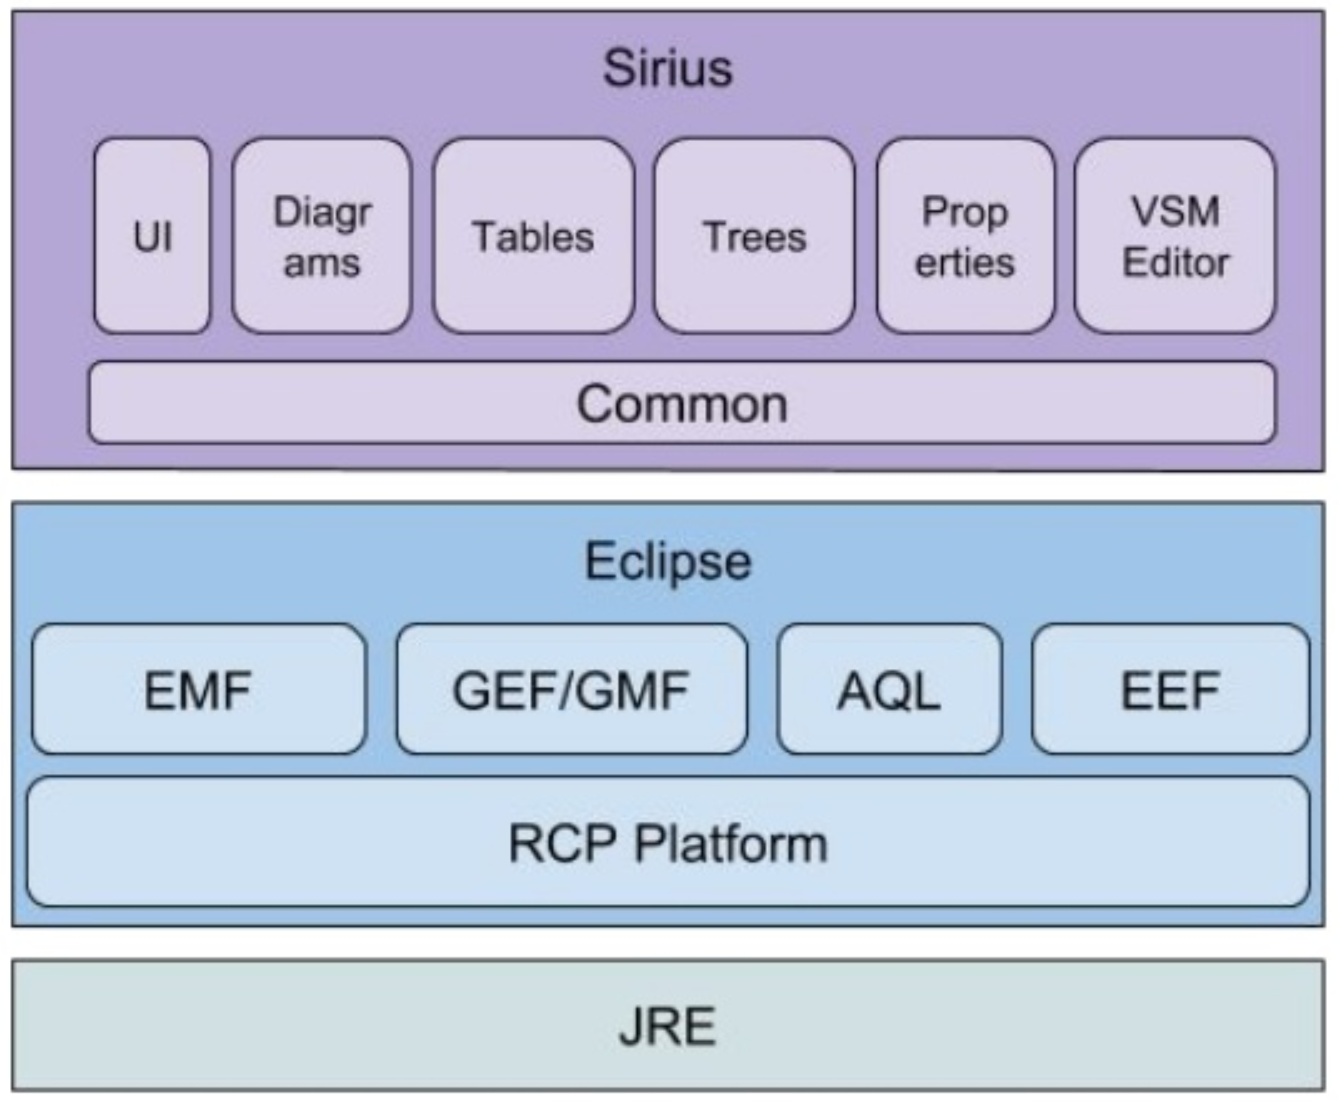
\includegraphics[width=\textwidth]{figures/Sirius_architecture}
  \caption[The Sirius Architecture]{The diagram shows the different components in Eclipse Sirius. The components on the top depend on the components below.~\cite[p.~36]{davidSiriusCon2018Sirius2018}.}\label{fig:sirius-architecture}
\end{figure}

\paragraph*{Using it} A developer creates Sirius specifications using the \gls{Eclipse}.
After a workbench is designed, the developer produces an Eclipse \emph{plugin} to distribute the graphical modeling tool. An end-user which edits model instances would install the plugin into their \gls{Eclipse}.

% When? Who? Why?

\subsubsection{Sirius Web}\label{sec:sirius-web}
% What is Sirius Web?
% When? Who? Why?

\paragraph*{What it is}
Sirius Web is an ongoing effort\footnote{As of 2020. It is supposed to be ready near the start of 2021.} to move the end-user editors of Sirius to the web.
The goal is to allow end-users to model with their browsers, instead of the \gls{Eclipse}.
Sirius Web will be \gls{open source}.
An illustration of Sirius Web's internal architecture is shown in \cref{fig:sirius-web-architecture}. Note that this is a work in progress, so the actual architecture may deviate once Sirius Web is released.
The end-user will only see the \emph{Sirius Web Frontend} (or \emph{Sirius \acrshort{RCP}}, which is the old Sirius in \cref{sec:sirius}).

Sirius Web does not use Theia, but its representations \textit{can} be shown in Theia.~\cite{neilmackenzieSiriusWebXText2020}

\paragraph*{Using it} A developer creates Sirius specifications in \emph{Eclipse Sirius} or \emph{Obeo Designer} as before. 
Then they deploy the specifications as a Sirius Web editor, instead of an Eclipse plugin.

\begin{figure}[htbp]  % order of priority: h here, t top, b bottom, p page
  \centering
  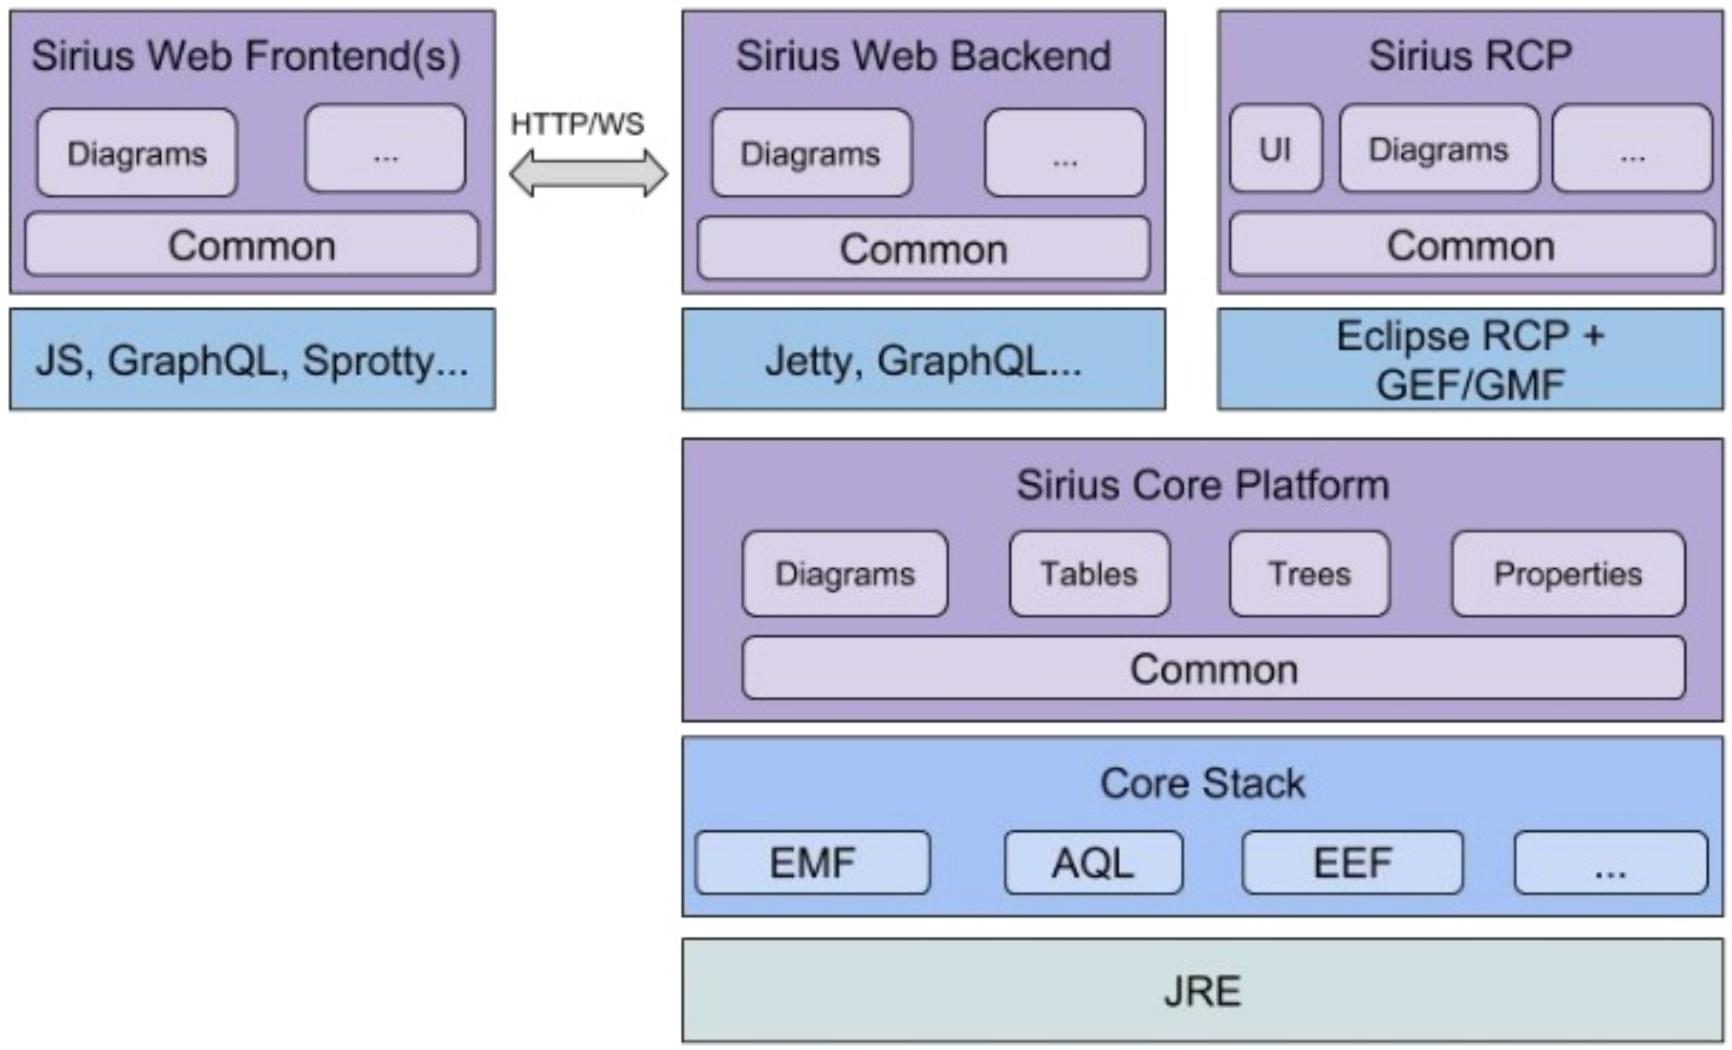
\includegraphics[width=\textwidth]{figures/Sirius-future-web-architecture}
  \caption[The Sirius Web Architecture]{The diagram shows the different components that will be in Sirius Web. Components on the top depend on components below.~\cite[p.~37]{davidSiriusCon2018Sirius2018}}\label{fig:sirius-web-architecture}
\end{figure}


% crossecore-generator
% More on the side of a genmodel alternative.
% https://github.com/crossecore/crossecore-generator
% TODO: write

\subsection{Ecore Editors}\label{sec:ecore-editors}

This section describes some of the existing editors for \gls{Ecore} models.
Most of them are provided in the \gls{Eclipse}.
They can be used to draw inspiration for new \gls{cloud} editors, and suggest functionalities and requirements that are needed.

\subsubsection{Sample Reflective Ecore Model Editor} %Default EMF Genmodel editor
A master-detail tree editor in \gls{Eclipse}.
It uses the \emph{reflective \acrshort{API}} of \gls{Ecore} to convert models into trees.
It is \gls{open source}\footnote{Sample Reflective editor source: \href{https://git.eclipse.org/c/emf/org.eclipse.emf.git/tree/plugins/org.eclipse.emf.ecore.editor}{https://git.eclipse.org/c/emf/org.eclipse.emf.git/tree/plugins/org.eclipse.emf.ecore.editor}.}
The source code lives in the \href{https://git.eclipse.org/c/emf/org.eclipse.emf.git/tree/plugins/org.eclipse.emf.ecore.editor/src/org/eclipse/emf/ecore/presentation/EcoreEditor.java}{org.eclipse.emf.ecore.editor} package, (indicating that it was generated by a \texttt{genmodel}\footnote{Some source code also has \texttt{@generated} annotations, confirming this.}).

A screenshot of the editor can be seen in \cref{fig:sample-reflective-ecore-model}.
It supports both models (\cref{sfig:sample-reflective-ecore-model-screenshot}) and model instances (\cref{sfig:sample-reflective-ecore-model-instance-screenshot}).

A relevant piece of the source code is the \texttt{ReflectiveItemProvider}\footnote{\href{https://git.eclipse.org/c/emf/org.eclipse.emf.git/tree/plugins/org.eclipse.emf.edit/src/org/eclipse/emf/edit/provider/ReflectiveItemProvider.java}{https://git.eclipse.org/c/emf/org.eclipse.emf.git/tree/plugins/org.eclipse.emf.edit/src/org/eclipse/emf/edit/provider/ReflectiveItemProvider.java}} from \texttt{org.eclipse.emf.edit}.
This code converts the model instances to text labels (\href{https://git.eclipse.org/c/emf/org.eclipse.emf.git/tree/plugins/org.eclipse.emf.edit/src/org/eclipse/emf/edit/provider/ReflectiveItemProvider.java#n390}{line 390}) and provides their icons (\href{https://git.eclipse.org/c/emf/org.eclipse.emf.git/tree/plugins/org.eclipse.emf.edit/src/org/eclipse/emf/edit/provider/ReflectiveItemProvider.java#n380}{line 380}), for display in a tree.
% https://git.eclipse.org/c/emf/org.eclipse.emf.git/tree/plugins/org.eclipse.emf.edit/model/Tree.ecore

\begin{figure}
    \centering
    \begin{subfigure}[b]{.45\textwidth}
        \centering
        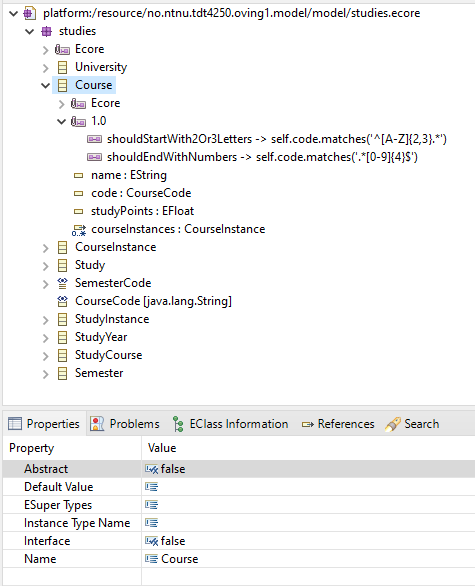
\includegraphics[width=\textwidth]{figures/ecore-sample-reflective-ecore-model-editor}
        \caption{A model opened in the editor.}
        \label{sfig:sample-reflective-ecore-model-screenshot}
    \end{subfigure}
    \hfill
    \begin{subfigure}[b]{.45\textwidth}
        \centering
        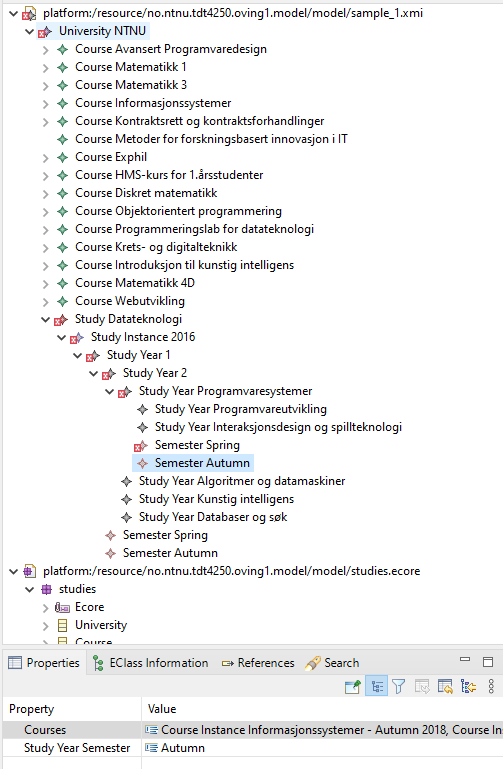
\includegraphics[width=\textwidth]{figures/ecore-sample-reflective-ecore-model-editor-instance.png}
        \caption{A \emph{dynamic instance} (\gls{XMI}) opened in the editor.}
        \label{sfig:sample-reflective-ecore-model-instance-screenshot}
    \end{subfigure}
    \caption{Screenshots of the Sample Reflective Ecore Model Editor in \gls{Eclipse}.}\label{fig:sample-reflective-ecore-model}
\end{figure}


\subsubsection{EMF Forms Ecore Editor} % EMF Forms based
The \emph{EMF Forms Ecore Editor} is based on \emph{EMF Forms}\footnote{\href{https://eclipsesource.com/blogs/tutorials/emf-forms-editors/}{https://eclipsesource.com/blogs/tutorials/emf-forms-editors/}}, a library to create form editors for \gls{Ecore} models.
It runs in \gls{Eclipse} and is \gls{open source}\footnote{EMF Forms source: \href{https://git.eclipse.org/c/emfclient/org.eclipse.emf.ecp.core.git/tree/bundles/org.eclipse.emfforms.editor.ecore}{https://git.eclipse.org/c/emfclient/org.eclipse.emf.ecp.core.git/tree/bundles/org.eclipse.emfforms.editor.ecore}.}.
The editor supports both \texttt{.ecore}, \texttt{.xmi} and \texttt{.genmodel} files.
It has a generic editor for all \gls{XMI} files\footnote{\emph{Generic XMI Editor} in \gls{Eclipse}.}, and specialized editors for ecore\footnote{\emph{Ecore Editor} in \gls{Eclipse}.} and genmodel.~\cite{eclipsesourceEMFFormsEditors2016}

A screenshot can be seen in \cref{fig:emf-forms-ecore-editor}.

\begin{figure}[htbp]  % order of priority: h here, t top, b bottom, p page
  \centering
  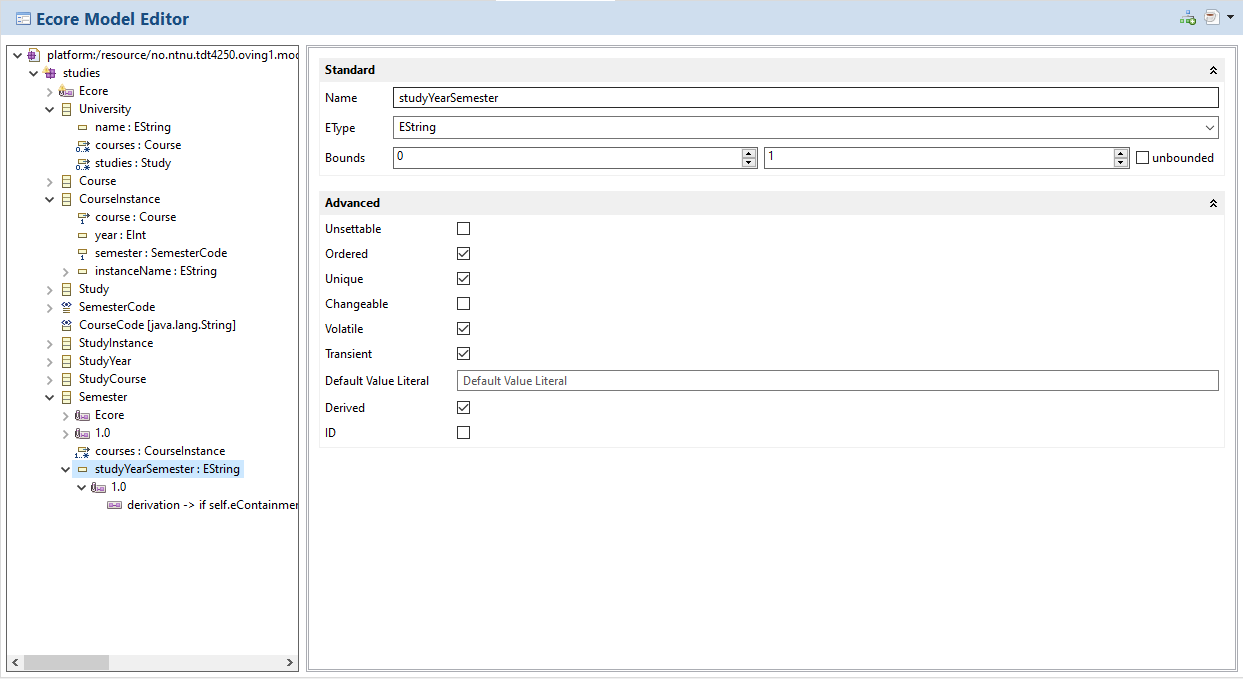
\includegraphics[width=\textwidth]{figures/ecore-eclipse-emf-forms-model-editor.png}
  \caption[EMF Forms Ecore Editor]{A screenshot of a model in the EMF Forms based Ecore Editor.}\label{fig:emf-forms-ecore-editor}
\end{figure}



\subsubsection{Ecore Tools} % Sirius based
The \emph{Ecore Tools} editor is based on Sirius (see \cref{sec:sirius}).
It displays diagrams as \gls{UML} Class Diagrams in the \gls{Eclipse}.
The editor is \gls{open source}\footnote{Ecore Tools source: \href{https://git.eclipse.org/r/plugins/gitiles/ecoretools/org.eclipse.ecoretools/}{https://git.eclipse.org/r/plugins/gitiles/ecoretools/org.eclipse.ecoretools/}.}

A screenshot of the Ecore Tools editor is shown in \cref{fig:ecore-tools-screenshot}.

\begin{figure}[htbp]  % order of priority: h here, t top, b bottom, p page
  \centering
  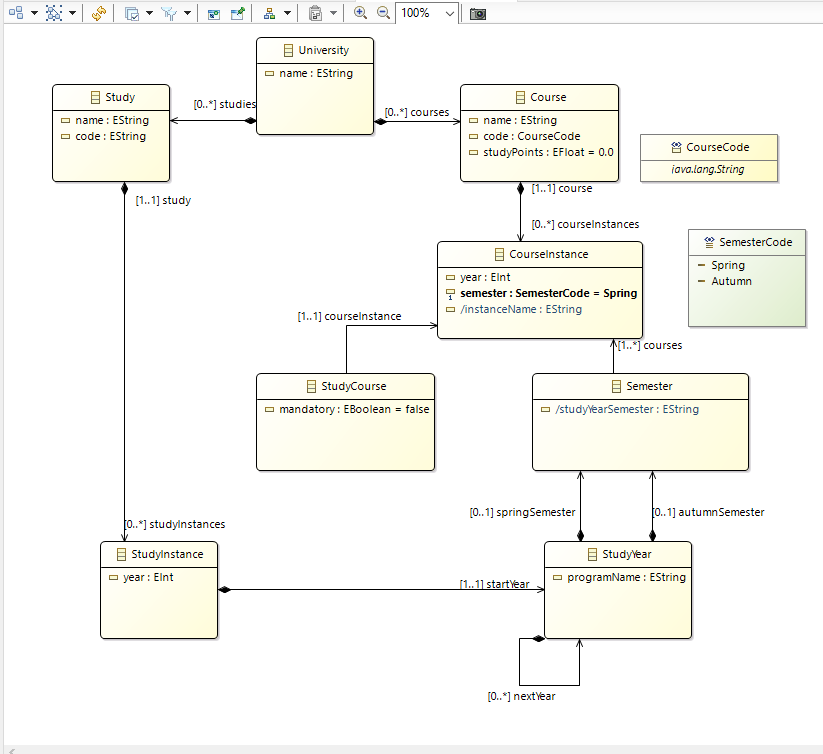
\includegraphics[width=\textwidth]{figures/ecore-eclipse-sirius-aird-graphical-editor.png}
  \caption[Ecore Tools Screenshot]{Ecore Tools in \gls{Eclipse} with a model opened.}\label{fig:ecore-tools-screenshot}
\end{figure}


\subsubsection{EMF.Cloud --- ecore-glsp}\label{sec:ecore-glsp} %Theia
The \emph{ecore-glsp} is an \gls{open source}\footnote{ecore-glsp source: \href{https://github.com/eclipse-emfcloud/ecore-glsp}{https://github.com/eclipse-emfcloud/ecore-glsp}.} \gls{Theia} \emph{Extension} (\cref{sec:theia-extension}) originally created by EclipseSource.
The project was donated to Eclipse EMF.Cloud.
It renders \gls{Ecore} models as diagrams, similar to Ecore Tools.

The extension is made using \gls{GLSP} (\cref{sec:glsp}) and Sprotty (\cref{sec:sprotty}).
When using the plugin, diagram layouts are persisted to a separate \texttt{.enotation} \gls{XMI} file.~\cite{camilleletavernierEclipseemfcloudEcoreglsp2020}

Although it only supports \gls{Theia} now, a developer using the \gls{GLSP} integration for \gls{VSCode} could possibly adapt it to a VSCode extension (see \cref{sec:vscode-extension}). A \gls{VSCode} integration library is created by EclipseSource\footnote{VSCode glsp integration source: \href{https://github.com/eclipsesource/glsp-vscode-integration}{https://github.com/eclipsesource/glsp-vscode-integration}.}.

The scope of the ecore-glsp library seems to extend beyond just diagrams.
The Github issues\footnote{Tree editor issue: \href{https://github.com/eclipse-emfcloud/ecore-glsp/issues/45}{https://github.com/eclipse-emfcloud/ecore-glsp/issues/45}.}\footnote{Model server issue: \href{https://github.com/eclipse-emfcloud/ecore-glsp/issues/28}{https://github.com/eclipse-emfcloud/ecore-glsp/issues/28}.}\footnote{Property view issue: \href{https://github.com/eclipse-emfcloud/ecore-glsp/issues/53}{https://github.com/eclipse-emfcloud/ecore-glsp/issues/53}.} indicate that the developers want to add a tree editor, property view, validation and a model server.
The issue for a tree editor suggest using the \emph{Theia Tree Editor} component (see \cref{sec:theia-tree-editor}).
However, if they add the Theia Tree Editor, the library \textit{may} lose compatibility with other \glspl{IDE} than \gls{Theia}, such as \gls{VSCode}.
Alternatively, the features will only be available in the \gls{Theia} client.

% CrossEcore Ecore editor
% https://github.com/crossecore/ecore-editor
% TODO: Write
% Typescript, ELKjs, Sprotty, Monaco and React
\subsection{Editor Extension Components}\label{sec:extension-components}

This section will describe the most relevant components, libraries or widgets for \acrshort{emf} in the \gls{cloud}, which can be used to create editor extensions.

Some of the libraries belong to \emph{EMF.Cloud}.
That is an Eclipse Foundation project umbrella for \gls{emf} tools for the \gls{cloud}\footnote{Eclipse EMF.cloud homepage: \href{https://projects.eclipse.org/projects/ecd.emfcloud}{https://projects.eclipse.org/projects/ecd.emfcloud}.}.


\subsubsection{Sprotty}\label{sec:sprotty}
Eclipse Sprotty is an \gls{open source}\footnote{Sprotty source: \href{https://github.com/eclipse/sprotty}{https://github.com/eclipse/sprotty}.} library to render diagrams in web browsers.
It uses Typescript, CSS and svg.
Sprotty can animate diagram changes.
The architecture is made with \gls{LSP} in mind, and supports having diagram data sent from a backend.
The library is configurable using dependency injection, and allows for adding custom nodes, edges and behaviors.
It also provides ``glue code'' for easy integration with \gls{LSP}, \gls{Theia} and \gls{ELK}.~\cite{smithEclipseSprotty2018}
An example of a sprotty diagram is shown in \cref{fig:sprotty-example}.

The library is mainly developed by TypeFox and EclipseSource, and managed by the Eclipse Foundation.~\cite{eclipsefoundationEclipseSprotty}

\begin{figure}[htbp]  % order of priority: h here, t top, b bottom, p page
  \centering
  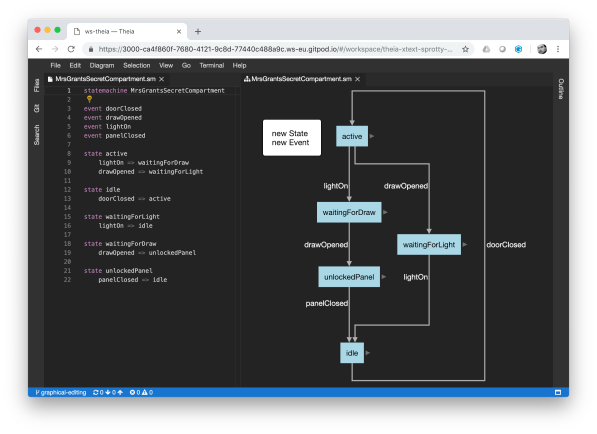
\includegraphics[width=\textwidth]{figures/sprotty-example.png}
  \caption[Sprotty Example]{This is a screenshot of Theia with a Sprotty diagram on the right side.~\cite{eclipsefoundationEclipseSprotty2020}}\label{fig:sprotty-example}
\end{figure}

\subsubsection{EMF.Cloud --- Theia Tree Editor}\label{sec:theia-tree-editor}
The \emph{Theia Tree Editor} is an \gls{open source}\footnote{Theia Tree Editor source: \href{https://github.com/eclipse-emfcloud/theia-tree-editor/tree/master/theia-tree-editor}{https://github.com/eclipse-emfcloud/theia-tree-editor/tree/master/theia-tree-editor}.} javascript framework for building tree editors in \gls{Theia}.~\cite{EclipseemfcloudTheiatreeeditor2020}
The framework is targeted at Theia Extensions (see \cref{sec:theia-extension}), and can not probably not be used in \gls{VSCode}\footnote{It \textit{may} be possible, if the VSCode extension pulls in the Theia \texttt{core}, however there could be dependencies to other \gls{Theia} \acrshortpl{API} as well.}.
The main reason is the dependence on tree structures defined in the Theia \acrshort{IDE} project itself (see \cref{fig:theia-tree-editor-node}).
To render the property form, it uses the \emph{JSON-Forms} library (\cref{sec:json-forms}).
Additionally, it uses \gls{React}.

\begin{figure}[htbp]  % order of priority: h here, t top, b bottom, p page
  \centering
  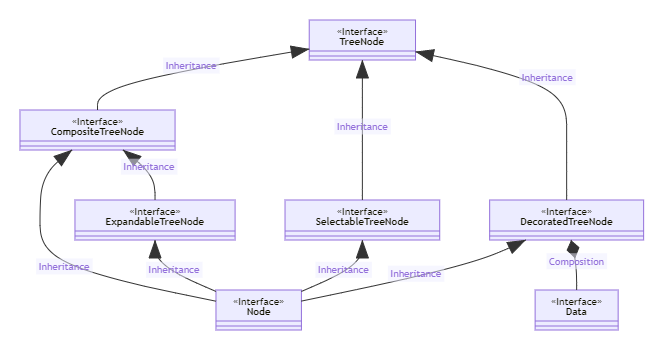
\includegraphics[width=\textwidth]{figures/theia-tree-editor-node.png}
  \caption[Theia Tree Editor Node's Class Hierarchy]{The Node class in Theia Tree Editor inherits multiple interfaces, all from the Theia \texttt{core} extension. Only \texttt{Node} resides in the Theia Tree Editor library itself.}\label{fig:theia-tree-editor-node}
\end{figure}

\subsubsection{JSON-Forms}\label{sec:json-forms}
JSON-Forms is an \gls{open source}\footnote{JSON-Forms source: \href{https://github.com/eclipsesource/jsonforms}{https://github.com/eclipsesource/jsonforms}.} javascript library by EclipseSource for creating HTML form editors.
A form is defined by two key elements: a \emph{data/JSON schema} and a \emph{UI schema}.
The \gls{JSON} schema defines the data types and validations for input.
The User Interface (UI) schema defines the visible \emph{form controls} (text fields, groups, labels) and binds them to a object property in the JSON schema.~\cite{eclipsesourceJSONForms}
For an example of how a form can look like, see \cref{fig:json-forms-example}.

A visual editor for JSON-Forms schemas exist at \href{https://github.com/eclipsesource/jsonforms-editor}{https://github.com/eclipsesource/jsonforms-editor}.

\begin{figure}[htbp]  % order of priority: h here, t top, b bottom, p page
  \centering
  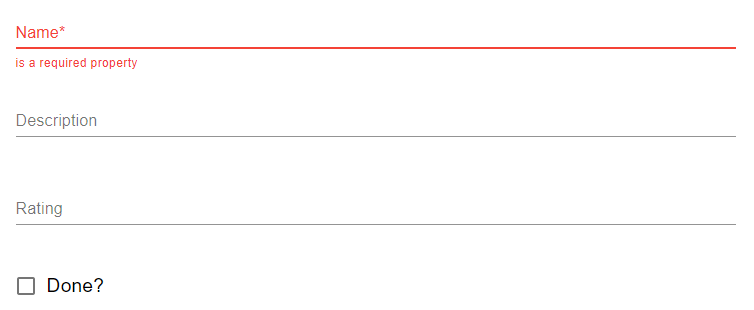
\includegraphics[width=.8\textwidth]{figures/json-forms-example}
  \caption[JSON-Forms Example]{An example of a form generated by JSON-Forms. It is displayed in a web browser.}\label{fig:json-forms-example}
\end{figure}

\subsubsection{EMF.Cloud --- Model Server}\label{sec:model-server}
The \emph{Model Server} is an \gls{open source}\footnote{Model Server source: \href{https://github.com/eclipse-emfcloud/emfcloud-modelserver}{https://github.com/eclipse-emfcloud/emfcloud-modelserver}.} java library and standalone web server.
It can discover and read \gls{Ecore} and \gls{XMI} files in a workspace folder.
Then the models can be provided as \gls{JSON} over a \gls{REST} \acrshort{API}, and changes to the models can be provided via \gls{WebSocket} subscriptions.~\cite{eugenneufeldEclipseemfcloudEmfcloudmodelserver2020}

A copy of the standalone \texttt{.jar} can be downloaded from a Maven Repository at \href{https://oss.sonatype.org/content/repositories/snapshots/org/eclipse/emfcloud/modelserver/org.eclipse.emfcloud.modelserver.example/0.7.0-SNAPSHOT/}{https://oss.sonatype.org/content/repositories/snapshots/org/eclipse/emfcloud/modelserver/org.eclipse.emfcloud.modelserver.example/0.7.0-SNAPSHOT/}.
(Note that the standalone seems to embed a coffee model example.
However, the implementation works with all \texttt{EObject}s and reads the \gls{Ecore} metamodel, so the use of the coffee model is not clear).
The \acrshort{API} provided can also serve \emph{JSON-Schema} and \emph{UI Schema}, which JSON-Forms in \cref{sec:json-forms} can consume.

The Model Server could be used in an extension or plugin (\cref{sec:extension-mechanisms}) as a backend child process, provided that the host operating system has a java runtime available.

%\subsubsection{Eclipse Edit} ?
% TODO: write
% From genmodel. Strictly not cloud, but could aid a backend.

\subsubsection{EMF.Cloud --- emfjson-jackson}
Originally, \emph{emfjson} was a project umbrella for \gls{emf} in the \gls{cloud}.
One part of emfjson, the \gls{JSON} serializer called \emph{emfjson-jackson} was donated to EMF.Cloud.
This is an \gls{open source}\footnote{Emfjson-jackson source: \href{https://github.com/eclipse-emfcloud/emfjson-jackson}{https://github.com/eclipse-emfcloud/emfjson-jackson}.} java library which uses the Jackson JSON library.\cite{guillaumehillairetEclipseemfcloudEmfjsonjackson2020}

% ecore.js ?https://github.com/emfjson/ecore.js
% Seems to be missing typescript definitions
% TODO: write

% crossecore-emfforms
% https://github.com/crossecore/crossecore-emfforms
% EMF Forms editor creator for web
% TODO: Write

% TODO: mention the glsp?
% TODO: Mention theia, eclipse, vscode?

% Che? Gitpod?
% TODO: Add missing sections
\section{Protocols}\label{sec:protocols}

This section will describe some of the protocols used by the editors in \cref{sec:editors} and extensions in \cref{sec:extension-components}.

\subsection{Language Server Protocol (LSP)}\label{sec:lsp}

\paragraph*{Goal} An \gls{IDE} often has to support many programming languages.
Most of the languages support some common features, such as autocomplete,  validation, definitions, references, renaming, selection etc..
The \gls{LSP} tries to separate language editor clients from language servers.
The clients are kept generic, while the language servers know the details for a programming language.~\cite{microsoftOverview}
This means a \gls{IDE} developer only needs to create \textit{one} editor, with generic \gls{LSP} support.
And a language developer only needs to create a language server.
If the language server adheres to the \gls{LSP} protocol, any \gls{LSP} client will automatically support it.
This is illustrated in \cref{fig:lsp-benefits}.

\begin{figure}[htbp]  % order of priority: h here, t top, b bottom, p page
  \centering
  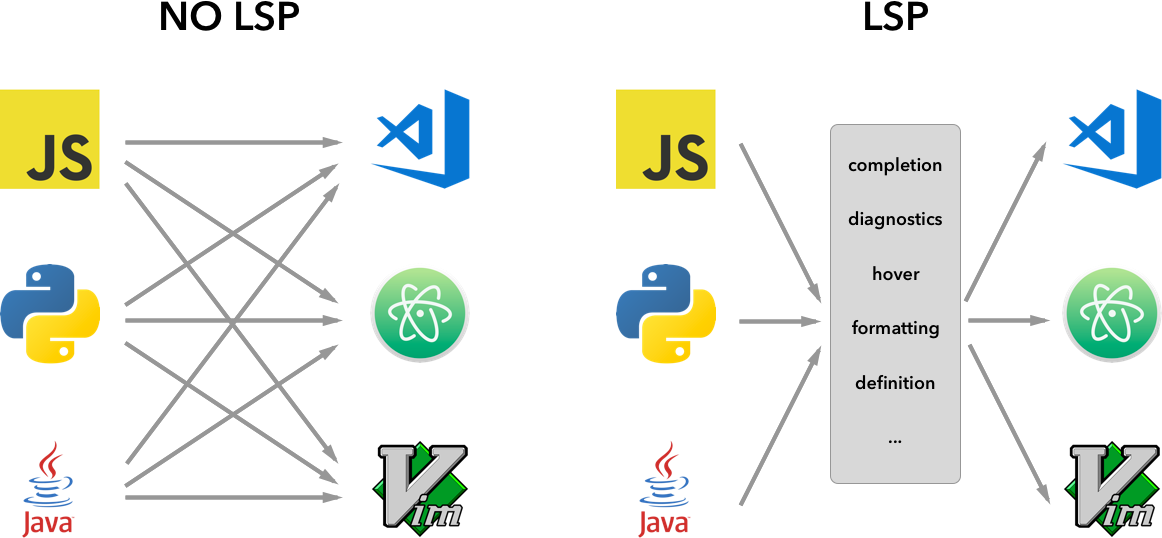
\includegraphics[width=\textwidth]{figures/lsp-languages-editors}
  \caption[LSP Benefits]{The benefits of using \gls{LSP}. There is no need for re-creating language support for every possible combination of editor and language.~\cite{microsoftLanguageServerExtension2020}}\label{fig:lsp-benefits}
\end{figure}


\paragraph*{Details}
The protocol is based on a \emph{Base protocol}, which has a \texttt{key-value} \emph{header} and a \emph{content} with \gls{JSON-RPC} (see \cref{fig:lsp-protocol}).

\begin{figure}[htbp]
  \centering
  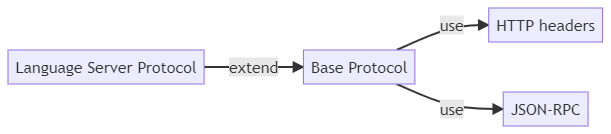
\includegraphics[width=\textwidth]{figures/lsp-protocol}
  \caption[The LSP Protocol]{The LSP protocol extends a Base protocol that uses HTTP headers and JSON-RPC content.}\label{fig:lsp-protocol}
\end{figure}

\paragraph*{The Base protocol}
The header fields conform to the HTTP specification\footnote{RFC-7230 at \href{https://tools.ietf.org/html/rfc7230\#section-3.2}{https://tools.ietf.org/html/rfc7230\#section-3.2}.} with regards to structure and formatting.

The Base protocol defines tree different message types that are sent in the \gls{JSON-RPC} content: \emph{Request}, \emph{Response} and \emph{Notification}.
There are also two key rules: every Request must be answered with a Response, and Notification does not need a Response.
The Base protocol provides a list of common error codes, extending the default error codes that \gls{JSON-RPC} provides.~\cite{microsoftLanguageServerProtocol2020}

The Base protocol defines a rule for Request and Notification methods as well: a method starting with \texttt{\$/} is protocol implementation specific and therefore optional, meaning a client or server can skip implementing it if the method is not suitable\footnote{The example given is cancellation of asynchronous tasks in a server that is synchronous.}.~\cite{microsoftLanguageServerProtocol2020}

Lastly, the Base protocol defines two Notifications: \texttt{\$/progress} and \texttt{\$/cancelRequest}.~\cite{microsoftLanguageServerProtocol2020}

\paragraph*{The Language Server Protocol}
The actual \emph{Language Server Protocol} itself is a large collection of \gls{JSON-RPC} Request, Response and Notification messages sent over the Base protocol.
The protocol assumes that \textit{one} language server is used for \textit{one} language client.~\cite{microsoftLanguageServerProtocol2020}
This means a language server can not be shared between multiple clients.

The protocol is tailored for textual languages and text documents.
It specifies a collection of data structures that should be used.
A central data structure is the \texttt{TextDocument}.
Inside a \texttt{TextDocument}, there can be \texttt{Location}s in the text, and \texttt{Range}s of text between two \texttt{Location}s.
Changing a \texttt{TextDocument} is done by constructing a \texttt{TextDocumentEdit}, which holds a list of text replacements in \texttt{TextEdit}s, and a pointer to a \texttt{TextDocument} version using a \texttt{VersionedTextDocumentIdentifier}.
A \texttt{TextEdit} has \texttt{Range} to edit and a string with the new text.~\cite{microsoftLanguageServerProtocol2020}
An illustration of the data structures are shown in \cref{fig:lsp-data-structures}.
Note that this is only a small subset of the data structures defined in \gls{LSP}\footnote{Most of the supported features are described at \href{https://code.visualstudio.com/api/language-extensions/language-server-extension-guide\#additional-language-server-features}{https://code.visualstudio.com/api/language-extensions/language-server-extension-guide\#additional-language-server-features}.}.

\begin{figure}[htbp]
  \centering
  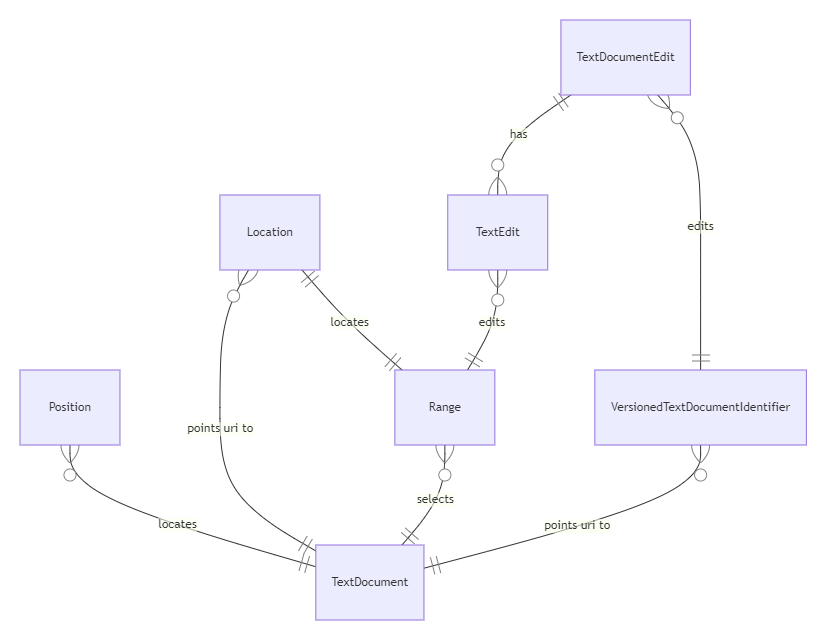
\includegraphics[width=\textwidth]{figures/lsp-textdocument-data}
  \caption[LSP Central Data Structures]{Central data structures in \gls{LSP}.}\label{fig:lsp-data-structures}
\end{figure}


\subsection{Graphical Language Server Platform (GLSP)}\label{sec:glsp}

% TODO: write
% https://github.com/eclipse-glsp/glsp#features

\subsection{JSON-RPC}

\paragraph*{Description}
\emph{JSON-RPC} is a stateless \acrfull{RPC} protocol.
That means it allows one process to call \emph{procedures} (methods, subroutines, functions) in another process.
The format for serializing the calls' data is \gls{JSON}.
A key design goal is to be a simple protocol.~\cite{json-rpcworkinggroupJSONRPCSpecification2010}

The protocol does not limit the \emph{transport mechanism} used, so \gls{JSON-RPC} could be sent inside the same process, across sockets, HTTP or any other form of message passing transport.~\cite{json-rpcworkinggroupJSONRPCSpecification2010}

\paragraph*{Protocol}
The main definitions are data structures and error codes.
\Gls{JSON-RPC} defines a \texttt{Request} and \texttt{Response} object.~\cite{json-rpcworkinggroupJSONRPCSpecification2010}

The Request must have an \texttt{id}, \texttt{method} name, \texttt{params} data structure and \texttt{jsonrpc} version field.
A Request without an \texttt{id} is a \texttt{Notification}, and will not get a Response back.~\cite{json-rpcworkinggroupJSONRPCSpecification2010}

The Response must have an \texttt{id}, \texttt{result} or \texttt{error} data structure, and a \texttt{jsonrpc} version field.~\cite{json-rpcworkinggroupJSONRPCSpecification2010}

% Architectures? Eclipse Plugin, Theia Extension
% TODO: Add missing sections

\chapter{Reviewed Research Questions}\label{chap:review-research-questions}

The research questions were presented in \cref{chap:research-questions}.
Some of them can be answered, at least to some extent, by the background material in \cref{chap:background}.

\section{The Old Research Questions}

\paragraph*{Modernizing \acrshort{mdd}}
First, lets look at \cref{rq:1}:
\begin{displayquote}
  How can we modernize \acrlong{mdd} Frameworks to appeal to the next generation of software developers, using recent developments in \gls{cloud} \acrshortpl{IDE}?
\end{displayquote}

It appears this modernization is already in progess.
With the introduction of \emph{Sirius Web} (\cref{sec:sirius-web}) and \emph{ecore-glsp} (\cref{sec:ecore-glsp}), \gls{Ecore} editors in \gls{cloud} based \glspl{IDE} are coming.
In addition, \gls{Ecore} code generation can already target web browsers using \emph{ecore.js} or \emph{crossecore-typescript}. % TODO: link to chapters


The use of more a more popular serialization format, \gls{JSON} instead of XML/\gls{XMI}, is being used to \textit{some} extent.
Most of the current efforts are still serializing to disk as \gls{XMI}, using only \gls{JSON} inside protocols for data transfer.
This \emph{could} be an advantage, however, to keep the interoperability between different tools.
Most of the developers' work is not done directly in these files, but instead with graphical interfaces. Therefore, this is perhaps not a big issue.


The biggest blocker right now is just implementation: not all features are supported yet.
Another concern is targeting only \gls{Theia}, as is the case for ecore-glsp with its use of Theia Extension (\cref{sec:theia-extension}).
This prevents usage in \gls{VSCode}\footnote{Although not a \gls{cloud} editor (yet? \href{https://github.com/features/codespaces}{https://github.com/features/codespaces}), it is very popular.~\cite{stackoverflowStackOverflowDeveloper2019}}, and also in Gitpod.
It could possibly be used in Che, by customizing the \gls{IDE} used\footnote{This may need help from a system administrator. Alternatively, a user can compile their own Docker image with a modified Theia instance, and specify it in a devfile.~\cite{maxshaposhnikIntroductionDevfile2020}}.


\paragraph*{Essential tools}
Next up is \cref{rq:2}:
\begin{displayquote}
  What tools are essential to use \acrlong{mdd} in the \gls{cloud}?
\end{displayquote}

The model editor seems like the obvious answer. 
Two different types of model editor were found.
There are tree and property editors, and graphical diagram editors.
These should support both the general \gls{Ecore} model and model instances.
Some editors also support the genmodel.

In addition, there is validation, comparison and code generation.
Of these, code generation seems most essential, and validation second.
The ongoing development in \cref{sec:ecore-editors} on ecore-glsp also seems to share this view: diagram editor first, then code generation, then validation last\footnote{Ecore-glsp already supports genmodel and EMF Codegen: \href{https://github.com/eclipse-emfcloud/ecore-glsp/issues/10}{https://github.com/eclipse-emfcloud/ecore-glsp/issues/10}.}.

Even though personal experience with \gls{emf} relied mainly on a tree editor, little focus has been on implementing \gls{Ecore} tree editors in the \gls{cloud} yet.
There is the generic Theia Tree Editor (\cref{sec:theia-tree-editor}), but it has not been applied to \gls{Ecore} yet.
A generic tree editor could work with models, model instances and the genmodel, making it a ``one solution to rule them all'', compared to diagram editors.
This is what \gls{Eclipse} has already, like the Sample Reflective Ecore Model Editor and the EMF Forms based editor.

Validation and code generation tools could be embedded in VSCode extensions as executables, and ran as VSCode commands or from a tree editor.
They do not require special user interfaces.

\paragraph*{A good tool}
Perhaps more on the side of \textit{usability}, or \textit{minimum viable product} requirements, is \cref{rq:3}:
\begin{displayquote}
  What does a good \gls{cloud} based tool for \acrlong{mdd} look like?
\end{displayquote}

Its characteristics are about its software architecture and functional requirements.
\textit{What does it do}?
And \textit{how} does the tool do something?

First off, flexibility seems to be key.
Flexibility and extensibility in the protocols used, and configurability with regards to details.
It is hard to define everything up front, so some leeway for tool developers is left in.
Custom protocol messages; optional functionality.
Using dependency injection in order to create an extendible system seems popular in this cohort of developers as well.
For example \gls{Theia}, Sprotty and \gls{GLSP} all do this.

Second is configuration. 
It is hard to predict everything, so exposing details as configuration options allows solutions to arise for unknown situations.
An example is \textit{java}: a lot of the \gls{emf} ecosystem exists as java code, and could be embedded as \texttt{.jar} files, but \emph{where is java installed} on the workspace operating system, and which java version?
With new environments like Gitpod and Che, some old assumptions do not hold\footnote{Example: you assume \texttt{java} can be invoked from the OS Path, but what if it is ran as a Docker container instead with \texttt{docker run}?}.

Third is to augment models instead of extending their serialization format.
Most of the tools store some extra data, like layout or options.
These pieces of information are stored in files separate from the \texttt{.ecore} model, such as \texttt{.aird}, \texttt{.json} and \texttt{.genmodel}.
Common is the usage of \gls{XMI}, but some use \gls{JSON}.

Fourth is a client-server separation, both because \gls{Theia} is distributed, but also to have reusable (generic) clients and reusable servers like \gls{LSP}.
Runtime dependencies may dictate how code is organized, for extensions that work across browsers, \gls{Electron} and \gls{Nodejs}.

% Fifth: using Ecore models internally? Used by some: Command API, Tree structure, maybe more

% Sixth: look for requirements in existing tools, like validation, undo/redo, refacotring, references, renaming etc?

\paragraph*{Reusing tools and architectures}
The last question is \cref{rq:4}:
\begin{displayquote}
  How can existing modeling tools and software architectures be reused in the new \gls{cloud} based modeling tool?
\end{displayquote}

It seems existing tools that can be run standalone as servers or command line tools can be reused.
For example, \gls{LSP} shows this, by letting language servers execute what they want internally, like existing compilers.
Bridging the gap between old programs and new could be done by exposing them over an \gls{API}, such as \gls{REST} or \gls{JSON-RPC}. The Model Server (\cref{sec:model-server}) does this, and hides away java and \gls{Ecore} model parsing behind a \gls{REST} \acrshort{API}.

% TODO: write some more. Architecture. LSP, Model server, generic frontends.

\section{Planned Contribution}%New Research Questions

\begin{questions}[leftmargin=1cm,resume]
  \item \emph{How can we design an Ecore master-detail tree editor that works in both VSCode and Theia, while reusing existing tools for Ecore such as codegen and validation?}\label{rq:21}
  \begin{questions}
    \item \emph{How can java applications be used in a VSCode extension?}\label{rq:22}
    \item \emph{How should the editor cooperate with multiple other tools that change the same underlying model?}\label{rq:23}
    \item \emph{What data is required for displaying a model as a tree?}\label{rq:24}
    \item \emph{How can a tree editor component be generic enough to support arbitrary user actions?}\label{rq:25}
    \item \emph{How can the user interface know the model well enough so the user is constrained from creating invalid Ecore trees?}\label{rq:26}
  \end{questions}
\end{questions}

\chapter{Method}

\paragraph*{How to answer the research questions}
To answer the sub-research questions \cref{rq:22} to \cref{rq:26}, a design and creation approach will be used.
Developing prototypes and testing them in the real environment can quickly remove doubts about feasibility, as long as the prototype works.
(In case a prototype fails to demonstrate a working approach, a new approach will have to be designed and tested in a new prototype.
If no new design can be made, then the background material needs further research.)

To answer the main question, \cref{rq:21}, an analysis of existing tools will form the requirements for the editor.
The findings from \cref{rq:22} to \cref{rq:26} will influence the solution, and existing architectures and protocols will also be used as inspiration.

The answer to \cref{rq:21} will be a design, like diagrams and requirements.
It will not be a full implemented software solution, because of the limited scope of this pre-master's thesis specialization project.
An implementation will instead be explored in the following master's thesis.

\paragraph*{Data generation method}
To find data that can answer the research questions, I will use documentation on the internet from \gls{open source} software related to modeling.
Discovering the related software and documentation will be done by:
\begin{itemize}
  \item exploring the Eclipse Foundation's project umbrellas for related software
  \item inspecting the source code of existing \gls{Eclipse} \gls{Ecore} editors (discussed in \cref{sec:ecore-editors})
  \item searching with internet search engines (Google, GitHub) for \gls{emf} related libraries
  \item viewing presentations from \emph{EclipseCon 2020}\footnote{This is a developer conference by Eclipse Foundation. The 2020 conference has an agenda that aligns very well with modeling in the \gls{cloud}.} about \gls{emf} modeling, Sirius Web (\cref{sec:sirius-web}), \acrshort{GLSP}
  \item ask questions during\footnote{The conference happened during this thesis, and was virtual, so this was possible.} or after EclipseCon to presenters or key personalities 
  \item inspecting GitHub organizations that contribute modeling projects, to see if they offer other related projects
  \item inspecting developer documentation, guides and wiki pages for software, to find related documents
  \item inspect software dependencies\footnote{Usually listed in files like \texttt{pom.xml} and \texttt{package.json}} in discovered libraries, to find other related libraries 
\end{itemize}

\paragraph*{Data analysis}
The results will be analyzed qualitative to give a clear view of the state of the art, current developments, possibilities for new development and insight into the architectures and protocols already in use.
Together, this will form the basis of a new tool's requirements and design.



% What is a good solution
%  - How it fits into an existing ecosystem

% TODO: write

% Software requirements for the results

% Solve RQ2.1 with prototype 1
% Solve RQ2.2 with model server
% Solve RQ2.3 with prototype 2
% Solve RQ2.4 with prototype 2
% Solve RQ2.5 with prototype 2 [WIP]

% Answer RQ2 with diagrams from design-doc of prototype 2?

\chapter{Results}

% Contribution

% Move the background material for an editor here?
% Keep titles, use pointers in background, detail furhter here.

% Prototypes?
% What was gotten out of the experiments?

% (non-)Functional requirements here?

% Someting wrt. RQs
\chapter{Evaluation}

% With regards to software requirements

\chapter{Discussion}

% Sketch out.
% With regards to research questions

% TODO: write

\chapter{Conclusion}

% Sketch out.

% Sketch out Evaluation, Discussion, Conclusion.
% Not main focus for pre-project.

\chapter*{\bibname}
\printbibliography[heading=none]


\appendix
%\chapter{Additional Material}
\label{app:additional}

Additional material that does not fit in the main thesis but may still be relevant to share, e.g., raw data from experiments and surveys, code listings, additional plots, pre-project reports, project agreements, contracts, logs etc., can be put in appendices. Simply issue the command \texttt{\textbackslash appendix} in the main \texttt{.tex} file, and make one chapter per appendix.

If the appendix is in the form of a ready-made PDF file, it should be supported by a small descriptive text, and included using the \texttt{pdfpages} package. To illustrate how it works, a standard project agreement (for the IE faculty at NTNU in Gjøvik) is attached here. You would probably want the included PDF file to begin on an odd (right hand) page, which is achieved by using the \texttt{\textbackslash cleardoublepage} command immediately before the \texttt{\textbackslash includepdf[]\{\}} command. Use the option \texttt{[pages=-]} to include all pages of the PDF document, or, e.g., \texttt{[pages=2-4]} to include only the given page range.

\cleardoublepage
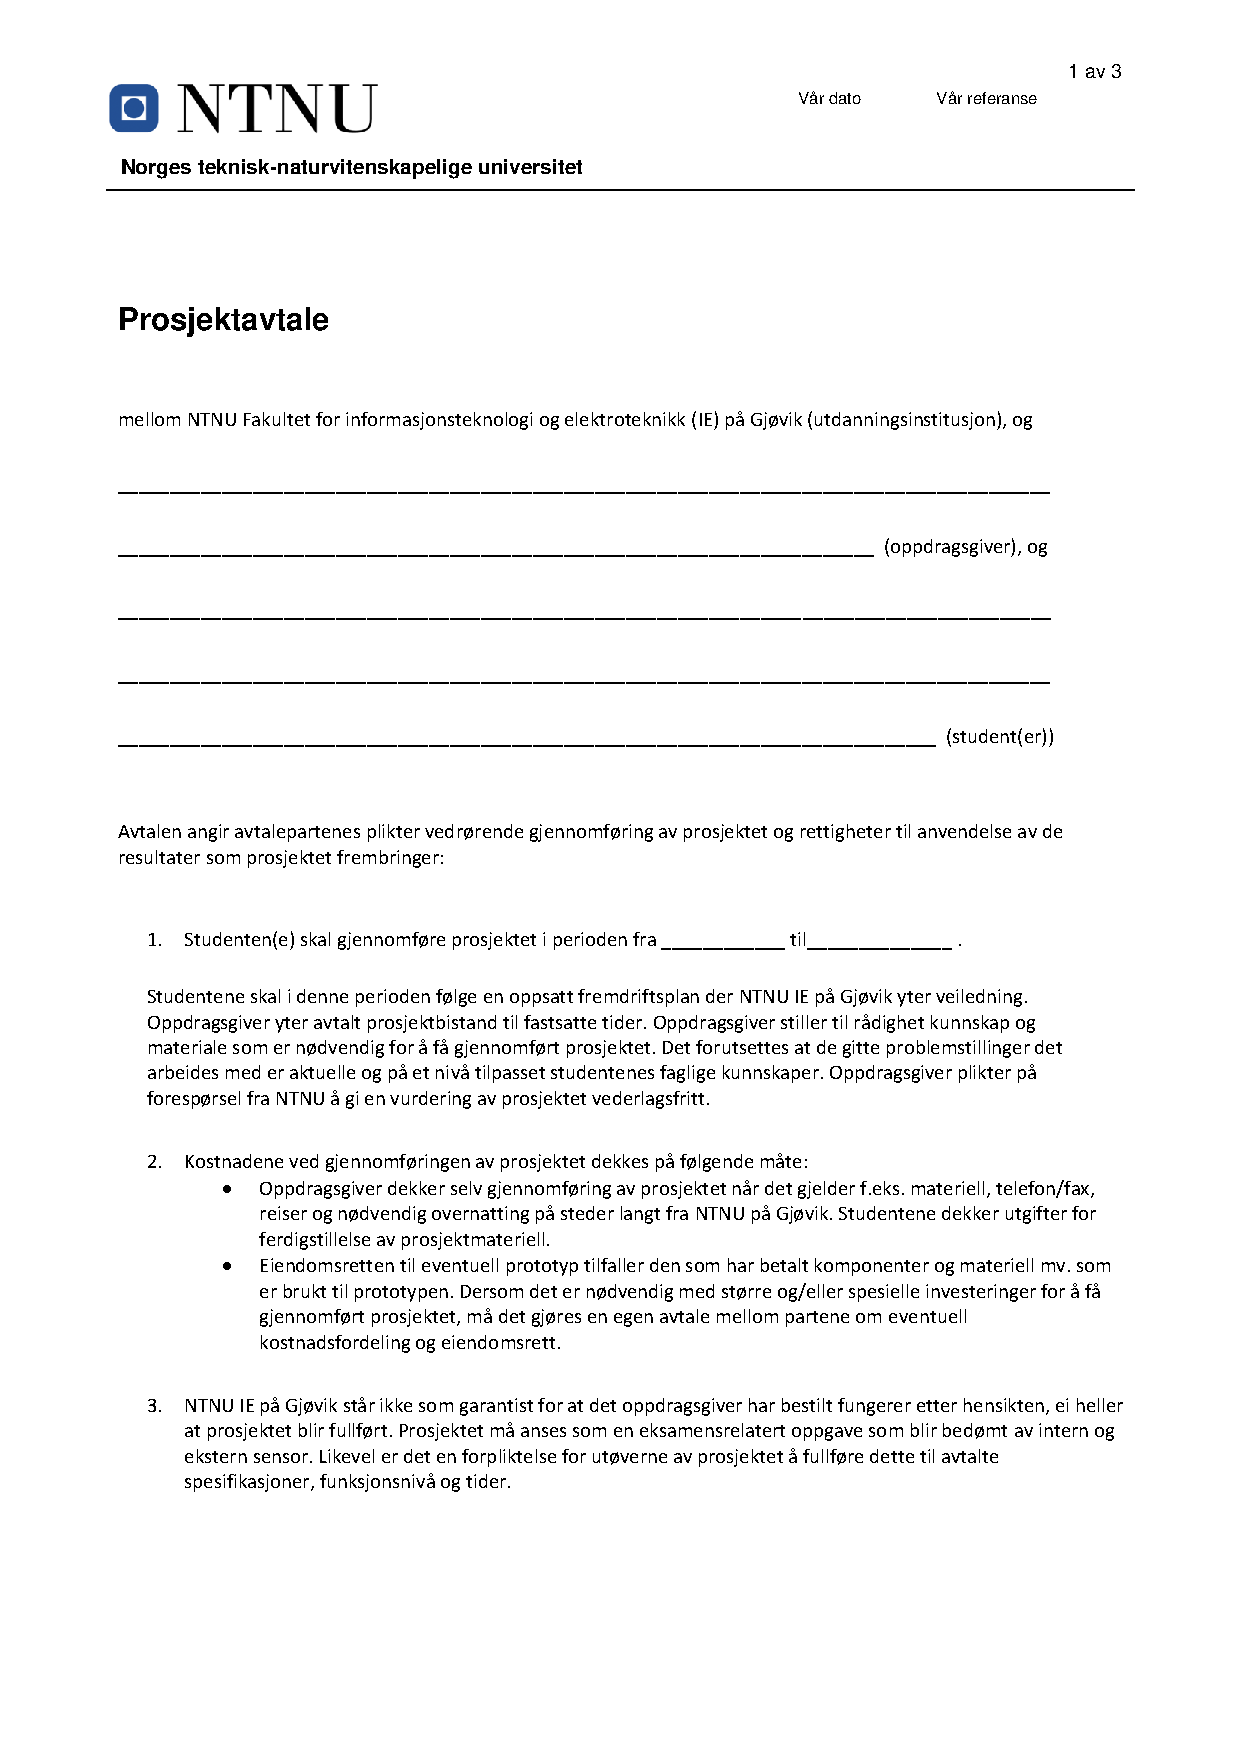
\includepdf[pages=-]{appendices/NTNUProsjektavtale.pdf}

\end{document}
